\documentclass[12pt,letterpaper]{book}
\usepackage[hyper]{uva-seas-thesis}
\usepackage{graphicx}
\usepackage{lineno}
\usepackage{todonotes}
\usepackage{siunitx}
\usepackage{booktabs}
\usepackage{tabulary}
\usepackage{appendix}
\usepackage{listings}
\usepackage{multirow}
\usepackage{pdfpages}
\linenumbers
\author{Andrew Ashworth}
\title{Versatile environmental monitoring platform}
\degree{Master of Science}
\program{Electrical Engineering}
\documenttype{thesis}
\graduationmonth{---}
\graduationyear{2015}
\begin{document}
\maketitle
\copyrightpage
%--------------------
\frontmatter
\begin{signatures}
\signature[Harry Powell]{Harry Powell, Advisor}
\signature[TBD]{TBD, Committee Chair}
\signature[TBD1]{TBD1}
\signature[TBD2]{TBD2}
\dean{James H. Aylor}
\end{signatures}
\dedication{To everyone who has helped me succeed}
\chapter{Abstract}

The ecoMOD project at UVA is an effort from the architectural school in designing low-cost, energy-efficient housing. In order to validate architectural design choices, the buildings must be instrumented post-construction. Building environment monitoring can give key feedback on energy and resource consumption. This work explores the design of a small, energy efficient, wireless sensing platform, along with a variety of sensor attachments. These attachments can detect: soil moisture and temperature, ambient light, and air temperature. By building functional prototypes, I demonstrate sensor operation and show how they can be used to monitor a residential building.
\tableofcontents
\listoftables
\listoffigures
%--------------------
\mainmatter
\chapter{Introduction}

The ecoMOD project is focused on creating sustainable, prefabricated housing units in partnership with local affordable housing organizations. These units are sustainable in that are environmentally responsive, with reduced energy, water, and maintenance costs compared to traditional housing stock. ecoMOD housing is aggressively affordable without cutting corners in construction, and strives to utilize the latest best practices in green, low-impact building and construction for a total cost of ownership that is markedly less than average. As a result, ecoOMOD housing has received numerous awards and accolades in the trade space\cite{Lau2013}.

\begin{figure}
\centering
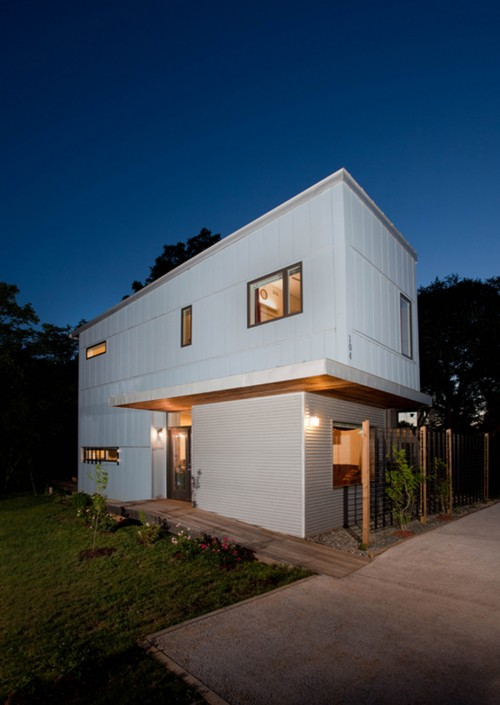
\includegraphics[width=0.3\linewidth]{./images/SFSmith_110602_8113-copy-500x705}
\caption{ecoMOD 4 in the evening\cite{Smith2011}}
\label{fig:SFSmith_110602_8113-copy-500x705}
\end{figure}

Historically, all ecoMOD housing has been extensively monitored with electronic instrumentation and networked for reasons of evaluating building performance. These sensors monitor important information such as ambient temperature, humidity levels, air quality, and electricity use. Data is collected and sent back to the University of Virginia for analysis. Residential buildings account for more than a third of total power consumption use (excluding transportation) in the United States\cite{EIA2015}. Quantifying the benefit of various design selections and operational behaviors is critical to analyzing the costs and benefits, and is the only way to provide targeted, effective feedback on methods of reducing construction cost and energy consumption.

Existing commercial monitoring solutions usually suffer the following problem: either they are excessively costly to install in the field, or are unreliable and difficult to integrate into existing data retrieval schemes. The ecoMOD project is no stranger to sensor deployments, having previously successfully opted to use expensive commercial solutions from vendors such as National Instruments or Onset Computers. Despite the cost, systems like the ones from National Instruments are being deployed year-after-year in many different buildings. They have seen extensive use in the commercial building industry due to the greater amount of capital and land involved. This demonstrates the clear value proposition of environmental monitoring systems. If these systems could be made cheaper, more accurate, and easier to use, homeowners and renters could objectively assess and audit their building performance metrics.

In this thesis, the design of a new sensing platform is presented. It is an extension of monitoring work that has been done continuously since the inception of the project, while introducing the foundations for future work in enabling environmental control by increasing platform capability. It is an evolutionary improvement over previous work done by Ernest Bowden in developing a development platform based around the MSP430 for the ecoMOD project\cite{Bowden2009}. The design was conducted with three major goals compared to previous work: easier deployments, increased robustness for experimentation, and retaining a low power consumption envelope. The designed node accomplishes this through three methods: use of 802.11 and Internet communication protocols for deployability, increased microprocessor speed and memory, and a very aggressive sleep schedule combined with a responsive, event-based software framework.

http://ieeexplore.ieee.org/xpls/icp.jsp?arnumber=1440950#ref_2
http://www.cmu.edu/gdi/docs/enhancing-electricity.pdf

\section{Related Work}

As mentioned previously, commercial sensor deployments from vendors such as National Instruments (NI) were used to instrument the first ecoMOD housing iterations\cite{Kidd2007}. However, as a business-focused product, the NI system was extremely expensive, with a small sensor deployment costing over \$10,000. Subsequent ecoMOD installations used a mixture of purpose-built electronics together with commercial-off-the-shelf (COTS) systems for monitoring. These included systems such as The Energy Detective (TED) from Energy Inc. (2009), and the Vantage Vue weather station from Davis Instruments. In general, this approach worked, but was difficult to integrate into a whole sensing and monitoring system, as each device had it's own unique interface and controls.

Failure to inter-operate is a well-known limitation of existing sensor network deployments. Commercially available devices use incompatible physical and application layer interfaces. At the physical layer, the most popular of these include IEEE 802.15.4, Bluetooth low-energy, and IEEE 802.11. At the application layer, Zigbee, Z-Wave, WirelessHART, and CoAP all enjoy significant mindshare. While there has been a push from industry players towards standardization of application and physical layer protocols, the market remains fragmented and many vendors lock customers in with proprietary and incompatible interfaces.

As the capabilities of microcontrollers increase, For a great deal of time, Internet Protocol (IP) was not used because it was considered inappropriate for use in distributed wireless sensor networks. Traditional mobile WiFi chips were targeted at laptops and cell-phones, which could be recharged on a daily or hourly basis. In addition, the protocol required too many computing resources as a proportion of microcontroller capability, especially at WiFi's higher data rates and encryption complexities. However, the problem has been solved from two sides. First, the steady advance of Moore's Law has brought down the cost in power and money of embedding computing capability. Second, the IETF has defined several reduced-functionality subsets of IP that can be implemented on smaller computers. These standards include IEEE 802.15.4, Routing over Low-Powered Lossy Networks (ROLL), and Constrained Application Protocol (CoAP). 

The device designed in this thesis utilizes a full 802.11 Internet stack along with an open hypertext interface. The adoption of IP for wireless sensor networks will speed their deployment and adoption. Communication compatibility between disparate devices will enable more competition between manufacturers, lower costs, and facilitate the creation of new services which span multiple sensor deployments. It will also allow the easy use of well-known Web technologies for aggregating and displaying sensor information.

\section{Related Devices}

\begin{figure}[h]
\includegraphics{images/telosB}
\caption{TelosB Sensor Mote\cite{1440950}}
\label{telosB}
\end{figure}

In wireless sensor network (WSN) research, a sensor node is popularly known as a "mote", which comes from the idea that future sensor nodes will be as ubiquitous as dust motes in an Internet cloud of devices. These existing devices have been used for many years to investigate new networking techniques and to collect data for environmental monitoring. As a result, the explored design space is similar to what is designed in this thesis. 

There are many commercially available motes. Interest in distributed sensing has only increased with the ongoing media coverage of the possibilities of the "Internet of Things", which is the idea that all future electronic devices will be seamlessly interconnected via the Internet due to rapidly declining costs in wireless technology. 

Typical mote characteristics are described in Table \ref{mote_characteristics}. Generally, they include several default sensors, a low-power transceiver, an 8-bit microcontroller, and tens of kilobytes of code data and storage. As development boards they have many pins broken out for easy expandability. While bare-metal programming of these devices is popular, two operating systems exist for these platforms, where new networking and application layer protocols are tested and researched. These are Berkeley's TinyOS, and the Swedish Institute of Computer Science's (SICS) ContikiOS.

\begin{table}[h]
\begin{tabular}{@{}lllll@{}}
\toprule
Processor & Platform Name & Speed (MHz) & Ram (Kb) & Transceiver \\ \midrule
TI MSP430 & TelosB & 8 & 10 & TI CC2420 \\
Atmel ATMega 128 & MICA & 8 & 4 & Atmel RF230 \\
MC1322x & Econotag & 26 & 128 & MC1322x \\
Atmel ATMega 128 & Waspmote & 14 & 8 & Varies \\ \bottomrule
\end{tabular}
\caption{Typical Mote Characteristics}
\label{mote_characteristics}
\end{table}

\section{Contributions}

This thesis describes a method for designing a development platform that allows for further research and monitoring into building performance envelopes. Power consumption is analyzed, and various methods for extending battery lifetime are explored. Chapter 1 explores the hardware design choices. Chapter 2 does a similar exploration of the firmware load. Chapter 3 presents a short overview of various energy trade-offs, followed by Chapter 4, which contains a conclusion and a summary of further work.
\chapter{Board Overview}

\section{Hardware Overview}
The designed board is a small, credit-card sized wireless sensor node. Temperature, humidity, and ambient light-levels are measured on-board, with the remaining micro-controller input-output broken out to a standard 0.1" pitch header for easy expandability. The board is based on the Texas Instruments CC3200, an ARM-M4 MCU and 802.11 radio SoC. 

\missingfigure{Board component-level block diagram}

The sensor node is designed to be small and non-invasive for easy deployment in residential and outdoor areas. The dimensions are sized to fit a standard Pelican 1010-series micro case, if a case is needed for outdoor, battery-powered operation. This case is rugged, waterproof, and made of transparent (optical and RF) polycarbonate.

The system is designed to run autonomously with little interaction by the user. Accordingly, there are no buttons or switches on the board, but if user interaction is required, they can be added to the 0.1" header.

The board is very flexible, and contains spare computational and memory capacity. The ARM-M4 microcontroller run at X MHz using an external crystal oscillator. It has Y program, memory, Z RAM, ADCs, blah, blah, add stuff from datasheet here. The current firmware load uses only AX kilobytes. New firmware loads can be easily inserted as a result.

\missingfigure{table of mcu characteristics}

The board microcontroller runs an event-based scheduling framework combined with a very simple, cooperative multitasking kernel, both sourced and ported from the GPL-licensed QP Framework\cite{qp framework}. There is very little hardware abstraction; peripherals and MCU features must be directly programmed and accessed. New events are easily created and assigned to the kernel scheduler, which schedules all tasks in a run-to-completion fashion. 

\section{Related Devices}





\chapter{Firmware Design}

Software has a critical impact on hardware design. Typically, for a project like this, either ContikiOS\cite{dunkels2011contiki} or TinyOS\cite{levis2005tinyos} would be chosen. Both of them are componentized operating systems that are the de-facto standard in wireless embedded systems research. However, neither was used for this project. Instead, the board runs a port of the QP Framework\cite{samek2008practical}, an event-based actor framework combined with a very simple, cooperative multitasking kernel. The advantage of choosing a bare-metal solution is that the kernel can be swapped out in the future depending on application requirements. If necessary, a pre-emptive kernel could be used in order to provide hard real-time guarantees to executing software. No such capability is supported by TinyOS or ContikiOS, because of the resource constraints imposed by the platforms they must support.

As a result of running directly on the microcontroller, there is very little hardware abstraction; peripherals and MCU features must be directly programmed and accessed via the ROM functions provided by the manufacture. New events are easily created and assigned to the QP scheduler, which schedules all tasks in a run-to-completion fashion. For this design, given that the hard real-time demands of the networking subsystem are serviced in a separate, dedicated microcontroller in the CC3200 package, a cooperative, non-preemptive kernel was judged to be appropriate. It is simple to implement, uses less stack and memory space, and does not suffer from the complexity of traditional preemptive real-time operating systems.
 
\section{Radio Duty Cycling, Data Aggregation, and Low Power Modes}

The node design is based on the following low duty cycle principle: the node is asleep for the majority of the time, wakes up quickly on an event, processes, and returns to sleep. For the lowest power consumption, the standby current and wakeup time (time to transition from sleep to active mode) must be minimized\cite{puccinelli2005wireless} since the the active portion of a sensor network application is typically extremely small\cite{shnayder2004simulating}. 

!!!Integration of programming, communication, storage, and sensing allows researchers to utilize more functionality and develop more robust systems.

\todo{reword above paragraph}

Wireless transmission and receive are the dominant power consumers in most battery-powered devices. The board designed here is no exception, with energy consumption dominated by the transceiver. A representative pie chart has been calculated assuming the transmission of one 8-bit sample per second, and is shown below.

\missingfigure{Relative power consumption of different subsystems}

From the pie chart, it is clear that the energy consumption bottleneck lies in the wireless radio. Several techniques can be used here to reduce power consumption: compressing the data stream, and employing burst transmissions.

\subsection{Burst Transmission}

A wireless sensor node spends most of time engaged in one-way communication. Very rarely does it need to be actively listening for commands from another device. If the node collects data at a fixed rate, then the radio on time can be minimized by buffering as much data as possible, and then transmitting it. At all other times, the radio can be placed in a power-saving idle or sleep mode. This trades power consumption for data latency and device memory.

Let the average power drawn by the radio during bursts be defined as $P_{B}$. Then, 

\begin{equation}
P_{B} = \frac{1}{T_{B}}[E_{oh} + T_{TX} +(T_{B}-T_{TX})P_{idle}]\cite{calhoun2005design}
\end{equation}

where $T_{B}$ is the period between bursts, $E_{oh}$ is the radio on/off power toggling cost, $T_{TX}$ is the transmission time, $P_{TX}$ is the power consumed during transmission, and $P_{idle}$ is the power consumed while the radio is asleep.



 
\section{Server Data Storage}
\section{Rest API Interface}
\section{Data Compression}
\subsection{Goulomb Coding}


\chapter{Conclusion}

The results described within have wide applicability to a wide variety of wireless devices. Compact size, easy-to-use software, and high energy efficiency are universally desired properties of most mobile devices today. RF transmission and receive can consume order of magnitudes more power than the signal processing for the workloads involved in environmental sensing due to the low computational complexity involved and the low current consumption of today's modern integrated sensors and microcontrollers. Techniques to reduce data transmission can drastically increase battery lifetimes. Similarly, 

Given the typical duty cycle and mode of operation of a wireless node, the wireless channel remains the dominant power consumer. 

\section{Future Work}

There remains a great deal of work to do in terms of firmware. As seen in the API appendix, currently only three querying commands are supported, and only for mains-powered boards. Battery-powered devices push data to the server, instead of the server pulling data from the sensor. No such server-side code has been written. In the future, it would be useful if battery-powered devices were accessed in the same way as mains-powered devices. This requires some method to emulate always-on behavior, as battery-powered devices may be asleep and unable to respond to a synchronously. One way to do this would be to have a mains-powered device act as a caching proxy for requests to battery-powered nodes. In fact, this is an area of open research\cite{Lu2011}. Additional and helpful software features would be to support automatic sensor discovery and configuration, perhaps by setting up server-mediated over-the-air updates with new sensor support whenever a new extension board is developed.
%--------------------
\backmatter
\bibliography{./bibliography/mybib}
\bibliographystyle{plain}

\begin{appendices}
\appendix{Hardware Schematics and Layout}

\missingfigure{place hardware schematics here}
\appendix{Source Code Listing}

\missingfigure{insert complete source code listing here}
\end{appendices}

\end{document}
